\documentclass[12pt,oneside,final]{ucthesis}

% extra package incluts
\usepackage{graphicx}
\usepackage[T1]{fontenc}
\usepackage[sc,osf]{mathpazo}
%\usepackage[nohead]{geometry}
\usepackage{hyperref}

\hypersetup{
  colorlinks = true,
  urlcolor = black,
  citecolor = blue
}

% XXX set correctly?
%\geometry{
%  body={6.5in, 8.5in},
%  left=1.0in,
%  top=0.5in,
%  bottom=0.75in
%}


% UCSB latex additions
\usepackage{amsmath}
%\usepackage{amssymb}
\usepackage{multirow}
%\usepackage{amsthm}
\newtheorem{thm}{Theorem}[chapter]
\newtheorem{cor}[thm]{Corollary}
\newtheorem{lem}[thm]{Lemma}

% Set off captions in smaller font
%\usepackage[labelfont={bf,up},margin=40pt,textfont={small}]{caption,subfig}

%% Uncomment this next section to make a nice pdf version have pretty internal hyperlinks
%\usepackage{hyperref}
% \hypersetup{
%     bookmarks=true,         % show bookmarks bar?
%     breaklinks=true,
%     unicode=false,          
%     pdftoolbar=true,        % show Acrobat’s toolbar?
%     pdfmenubar=true,        % show Acrobat’s menu?
%     pdffitwindow=false,     % window fit to page when opened
%     pdfstartview={FitH},    % fits the width of the page to the window
%     pdftitle={Wavelet analysis of stochastic circadian oscillators},    
%     pdfauthor={Richard harang},     % author
%     pdfnewwindow=true,      % links in new window
%     colorlinks=true,        % false: boxed links; true: colored links
%     linkcolor=red,          % color of internal links
%     citecolor=green,        % color of links to bibliography
%     filecolor=magenta,      % color of file links
%     urlcolor=cyan           % color of external links
% }


\begin{document}

\title{Title of the disseration goes here}
\author{Shaun C. Walbridge}

\report{Thesis}
\degree{Master of Arts}
\degreemonth{September}
\degreeyear{2012}
\approvalmonth{September}
\approvalyear{2012}

\chair{Steven D. Gaines}
\committeeII{Krzysztof W. Janowicz}
\committeeIII{Benjamin S. Halpern}
\nummembers{3}
\field{Ecology, Evolution and Marine Biology}
\campus{Santa Barbara}

\maketitle

\begin{frontmatter}

  %% Template pages
  \approvalpage 
  \copyrightpage

  %% Dedication
%   \begin{dedication}
%     \null\vfil{%\large
%       \hspace{\stretch{1}}
%       \begin{minipage}{3.2in}
%         \begin{center}
%           Dedicated to a better world.
%         \end{center}
%       \end{minipage}
%     } \vfil\null
%   \end{dedication}

  %% Acknowledgements
  \begin{acknowledgements}
    \addcontentsline{toc}{chapter}{Acknowledgements} 

    No work is the act of one alone, and this thesis is no exception. This thesis would not be possible without the thoughts and guidance of many. I owe the idea to Ben Halpern, without which I wouldn't have thought twice about shipping. The whole Gaines lab, including Dr. Steven Gaines himself, have been tremendously supportive, even when it required rose-colored glasses to see the connections between our work. The National Center for Ecological Analysis and Synthesis (NCEAS) has provided me with both the intellectual and technical means to carry out this work. Mark Schildhauer and Jim Regetz have helped me see new ways of marrying technology to science. The feedback from NCEAS postdocs, including Jennifer Balch, Jai Rangnathan, Carrie Kappel, and Darren Hardy have left this work richer. NCEAS staff member Ben Best has been a wonderful resource for understanding the ecological context of shipping. Megan McKenna and Steve Katz were gratious enough to share with me an actual application area for this information, and taught me much about how to intepret ship-borne observations. The manuscript is improved thanks to the thoughtful feedback of Oliver Soong. I am indebted to Dawn Wright, for seeing me through the fire, and supporting me through the transition between academia and industry. Thanks to my family and friends, for being there, even when they didn't understand what I was working on, or why anyone would care. And lastly, thanks to my fiancée, Jessica Phillips, who has helped me in too many ways to list.

    \setlength{\epigraphwidth}{.9\textwidth}
    \setlength{\epigraphrule}{0pt}
    \epigraph{\textit{If you want to build a ship, don't drum up the men to gather wood, divide the work and give orders. Instead, teach them to yearn for the vast and endless sea.}}
             {---\textsc{Antoine de Saint-Exupéry}}


  \end{acknowledgements}
\ssp

\dsp

  %% Abstract

  \begin{abstract}
    \addcontentsline{toc}{chapter}{Abstract} 
    Here is where the abstract goes.
%    \abstractsignature
  \end{abstract}



%%% Local Variables: 
%%% mode: latex
%%% TeX-master: "MAIN"
%%% End: 

	\tableofcontents
	\listoffigures
	\listoftables
\end{frontmatter}

\dsp

% individual chapters

\chapter{Introduction}
\label{cha:introduction}

This is chapter 1.  




%%% Local Variables: 
%%% mode: latex
%%% TeX-master: "MAIN"
%%% End: 

\chapter{A Theory of Portals}
\label{cha:portal-theory}

This is chapter 2.

%%% Local Variables:
%%% mode: latex
%%% TeX-master: "MAIN"
%%% End:


%%%%%%%%%%%%%%%%%%%%%

\part*{\addcontentsline{toc}{part}{Appendices}Appendices}
\chapter*{}
\appendix
%\appendix{}
%\gdef\thesection{Appendix \Alph{section}}

\chapter{Movement Modeling}
\label{sec:movement-modeling-appendix}

% XXX copy and paste job, include details here.... tools used? DETAILED APPROACH.
Each vessel track was rasterized to both an 90 arcsecond grid (\textasciitilde{}5.5km at the equator) and an equal area grid in the Hobo Dyer projection (Figure \ref{fig:eu-cargo-density}). The latter case assures that the density function is computed on grid cells representing the same area for each cell, unlike the geographic grid where area varies by latitude. A vessel is counted only once for each cell it passes through, as the focus here on overall movement patterns, and this criteria helps de-emphasize vessels with limited movement. Each raster vessel track was combined using simple map algebra to produce density maps for both the AIS and VOS data, for each of our vessel classes. % XXX Oliver: A passing cargo ship is comparable to a ferry crisscrossing the same spot continuously every day?  Not that you should do this, but somebody might wonder.

Maps produced in ArcGIS and Quantum GIS.

gdal_rasterize did the rasterization step

gdal_add, custom python code combined the results

paralellized in Python.

% Bresenham's line algorithm used for rasterizing the tracks. Only counted a ship moving through a single cell once to get movement patterns v. dockage

% XXX built spatial indexes and reordered the data on disk to match for performance.


\chapter{Record Linkage}
\label{sec:record-linkage-appendix}

The Jaro-Winkler formula is defined in two steps. First, The Jaro distance, $d_j $, is defined as:

% good code-based illustration at: http://www.gettingcirrius.com/2011/01/calculating-similarity-part-2-jaccard.html

\begin{equation}
  d_j = \left\{
  \begin{array}{l l}
    0 & \text{if }m = 0 \\ 
    \frac{1}{3}\left(\frac{m}{|s_1|} + \frac{m}{|s_2|} + \frac{m-t}{m}\right) & \text{otherwise} \end{array} \right.
\end{equation}

Where:

m = number of matching patterns
t = number of transposed characters
|s1| = length of first string
|s2| = length of second string

Two characters are considered matching when they are no further apart than:
\begin{equation}
  \left\lfloor\frac{\max(|s_1|,|s_2|)}{2}\right\rfloor-1
\end{equation}

The second component, added by Winkler, preferentially weights strings which match from the beginning, set by the prefix length $ l $.  Thus, the Jaro-Winkler distance is defined:

\begin{equation}
  d_w = d_j + (\ell p (1 - d_j))
\end{equation}

Where $ p $ is a constant scaling factor to adjust for the strength of common prefixes. In its usage here, $ p = 0.1 $ and $ l = 4 $.



\chapter{Tables}

\begin{table}[htbp]
  \begin{tabular}{lr}
    Attribute & Accuracy \\
    \hline
    Location (fixed from GPS signal) & $\simeq$10 meter accuracy) \\
    Timestamp (on broadcast) & $\simeq$100 ms \textit{radio transmission \& processing latency}\\
    Name \\
    Call Sign \\
    Maritime Mobile Service Identity (MMSI) \\
    Heading \\
    Speed \\
    Destination & \textit{rarely valid}
  \end{tabular}
  \caption[AIS broadcast attributes]{AIS broadcast attributes. Update frequency depends on ship speed, but varies between a minimum of a record every 2 seconds for quickly moving vessels, to once per 3 minutes for moored vessels. Additional attributes are available, but infrequently used.}
  \label{table:ais-broadcast-attributes}
\end{table}

% had this as a list, also some hackery with unnesting class data:
% select distinct(trim(both from unnest(class))), count(*) from clean.ships where validation_class = 'tanker' and validation_score > 0 and obs_count > 0 GROUP BY class ORDER BY btrim DESC;ships=# select distinct(trim(both from unnest(class))), count(*) from clean.ships where validation_class = 'tanker' and validation_score > 0 and obs_count > 0 GROUP BY class ORDER BY btrim DESC;

\begin{longtable}{l|l|l}
\hline \multicolumn{1}{|c|}{\textbf{Type}} & \multicolumn{1}{c|}{\textbf{Sub-type}} & \multicolumn{1}{c|}{\textbf{Vessels}} \\ \hline 
\endfirsthead

%\multicolumn{3}{c}%
%{{\bfseries \tablename\ \thetable{} -- continued from previous page}} \\
\hline \multicolumn{1}{|c|}{\textbf{Type}} &
\multicolumn{1}{c|}{\textbf{Sub-type}} &
\multicolumn{1}{c|}{\textbf{Vessels}} \\ \hline 
\endhead

%\hline \multicolumn{3}{|r|}{{Continued on next page}} \\ \hline
\endfoot
    cargo & cargo ship & 30355 \\
          & merchant & 2919 \\
          & bulk carrier & 1338 \\
          & container ship & 669 \\
          & general cargo & 608 \\
          & vehicle carrier & 56 \\
    tanker & tankship & 10460 \\
           & tanker   & 8731 \\
           & oil tanker & 1312 \\
           & liquefied gas carrier & 112 \\
           & chemical carrier & 39 \\
    other & merchant & 17460 \\
          & other ship & 9421 \\
          & unspecified & 4580 \\
          & motor boat & 4231 \\
          & inland waterways & 3825 \\
          & sloop & 2799 \\
          & reserved for future use & 2164 \\
          & all other activities & 1345 \\
          & reserved for regional use & 712 \\
  support & pusher/tug & 4392 \\
          & tug & 7885 \\
          & towing vessel & 2747 \\
          & supply vessel & 1501 \\
          & service vessels & 1388 \\
          & trawler & 1056 \\
          & dredger & 995 \\
          & vessel engaged in dredging or underwater operation & 776 \\
          & pilot vessel & 685 \\
  pleasure & pleasure/leisure & 22013 \\
           & pleasure & 14573 \\
           & pleasure craft & 7290 \\
           & sailing vessel & 5527 \\
           & yacht & 8214 \\
  fishing & fishing vessel & 11110 \\
          & fishing boat & 8454 \\
          & fishing industry & 5767 \\
          & fishing & 3213 \\
  passenger & passenger ship & 6478 \\
            & ferry & 704 \\
  high-speed & high-speed craft & 658 \\
             & high speed craft & 520 \\
  authority & sar-vessel & 699 \\
            & search and rescue vessel & 609 \\
            & rescue vessel & 102 \\
  \caption[Detailed ship classes]{Detailed ship class breakdown. Classes come from observationsgT}
  \label{table:ship-class-breakdown}
\end{longtable}

%\newpage
%\chapter{Source Code}
%\label{sec:source-code}

% include SOME python code here -- our AIS parser, what else?
% steps: download AIS
% parse ais
% insert AIS into DB, formalize
% download & parse ship databases

%All code used to generate the project is available at https://github.com/scw/ais-kml-parser. The full code is omitted from this document, due to length restrictions.

%\texttt{aiskml.py}:
%\inputminted[linenos,
%             numbersep=5pt,
%             frame=lines,
%             framesep=2mm]{r}{../code/kml/aiskml.py}

%\texttt{parsekml.py}:
%\inputminted[linenos,
%             numbersep=5pt,
%             frame=lines,
%             framesep=2mm]{r}{../code/kml/parsekml.py}

\chapter{Figures}
\label{sec:figures}

\begin{figure}[htbp]
  \centering
  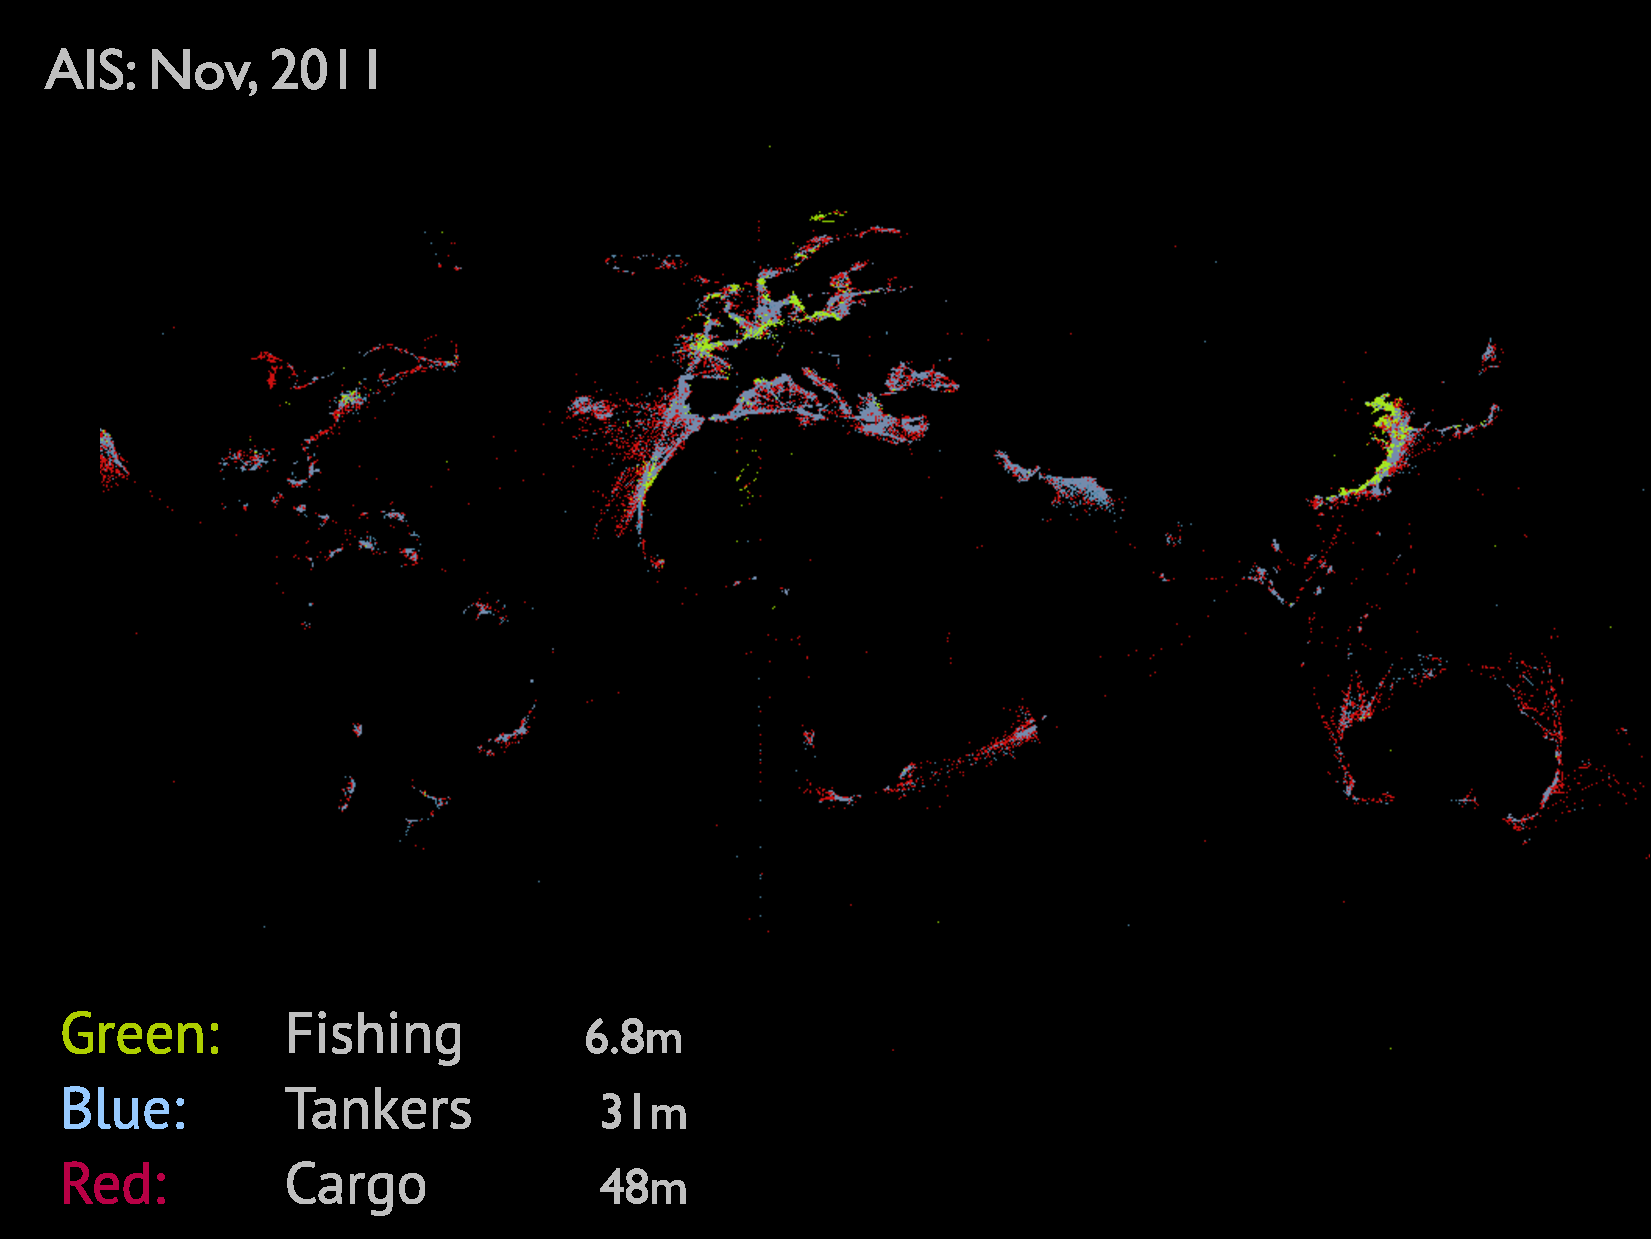
\includegraphics[width=160mm]{figures/ais-nov-2011.pdf}
  \caption[AIS observations, November 2011]{Raw AIS observations, November 2011. Note the observations located in the Hoggar Mountains in Algeria.}
  \label{fig:ais-obs-nov-2011}
\end{figure}

% show our image of invalid 'on land' ships in the harbor of long beach?
\begin{figure}[htbp]
  \centering
  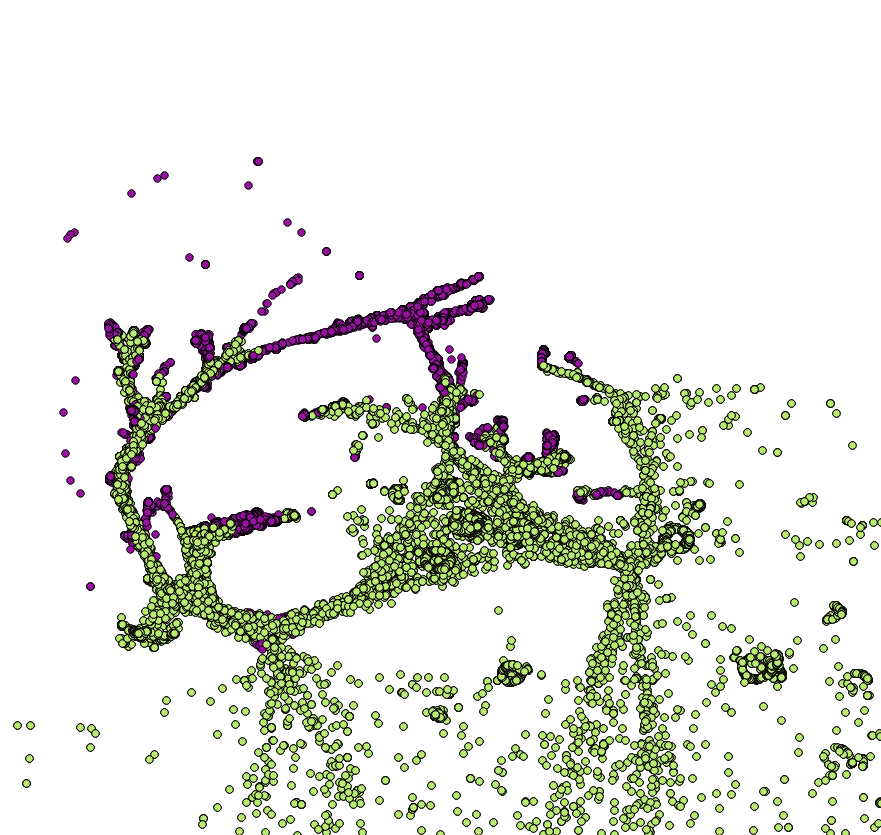
\includegraphics[width=140mm]{figures/example-long-beach-harbor-validation.png}
  \caption[Long beach harbor, validation example]{Long Beach Harbor, California. Points shown here in purple are 'on land', but most of these on-land observations are actually parts of the harbor.} % XXX Oliver: a little context here?
  \label{fig:longbeach-validation}
\end{figure}


\begin{figure}[htbp]
  \centering
  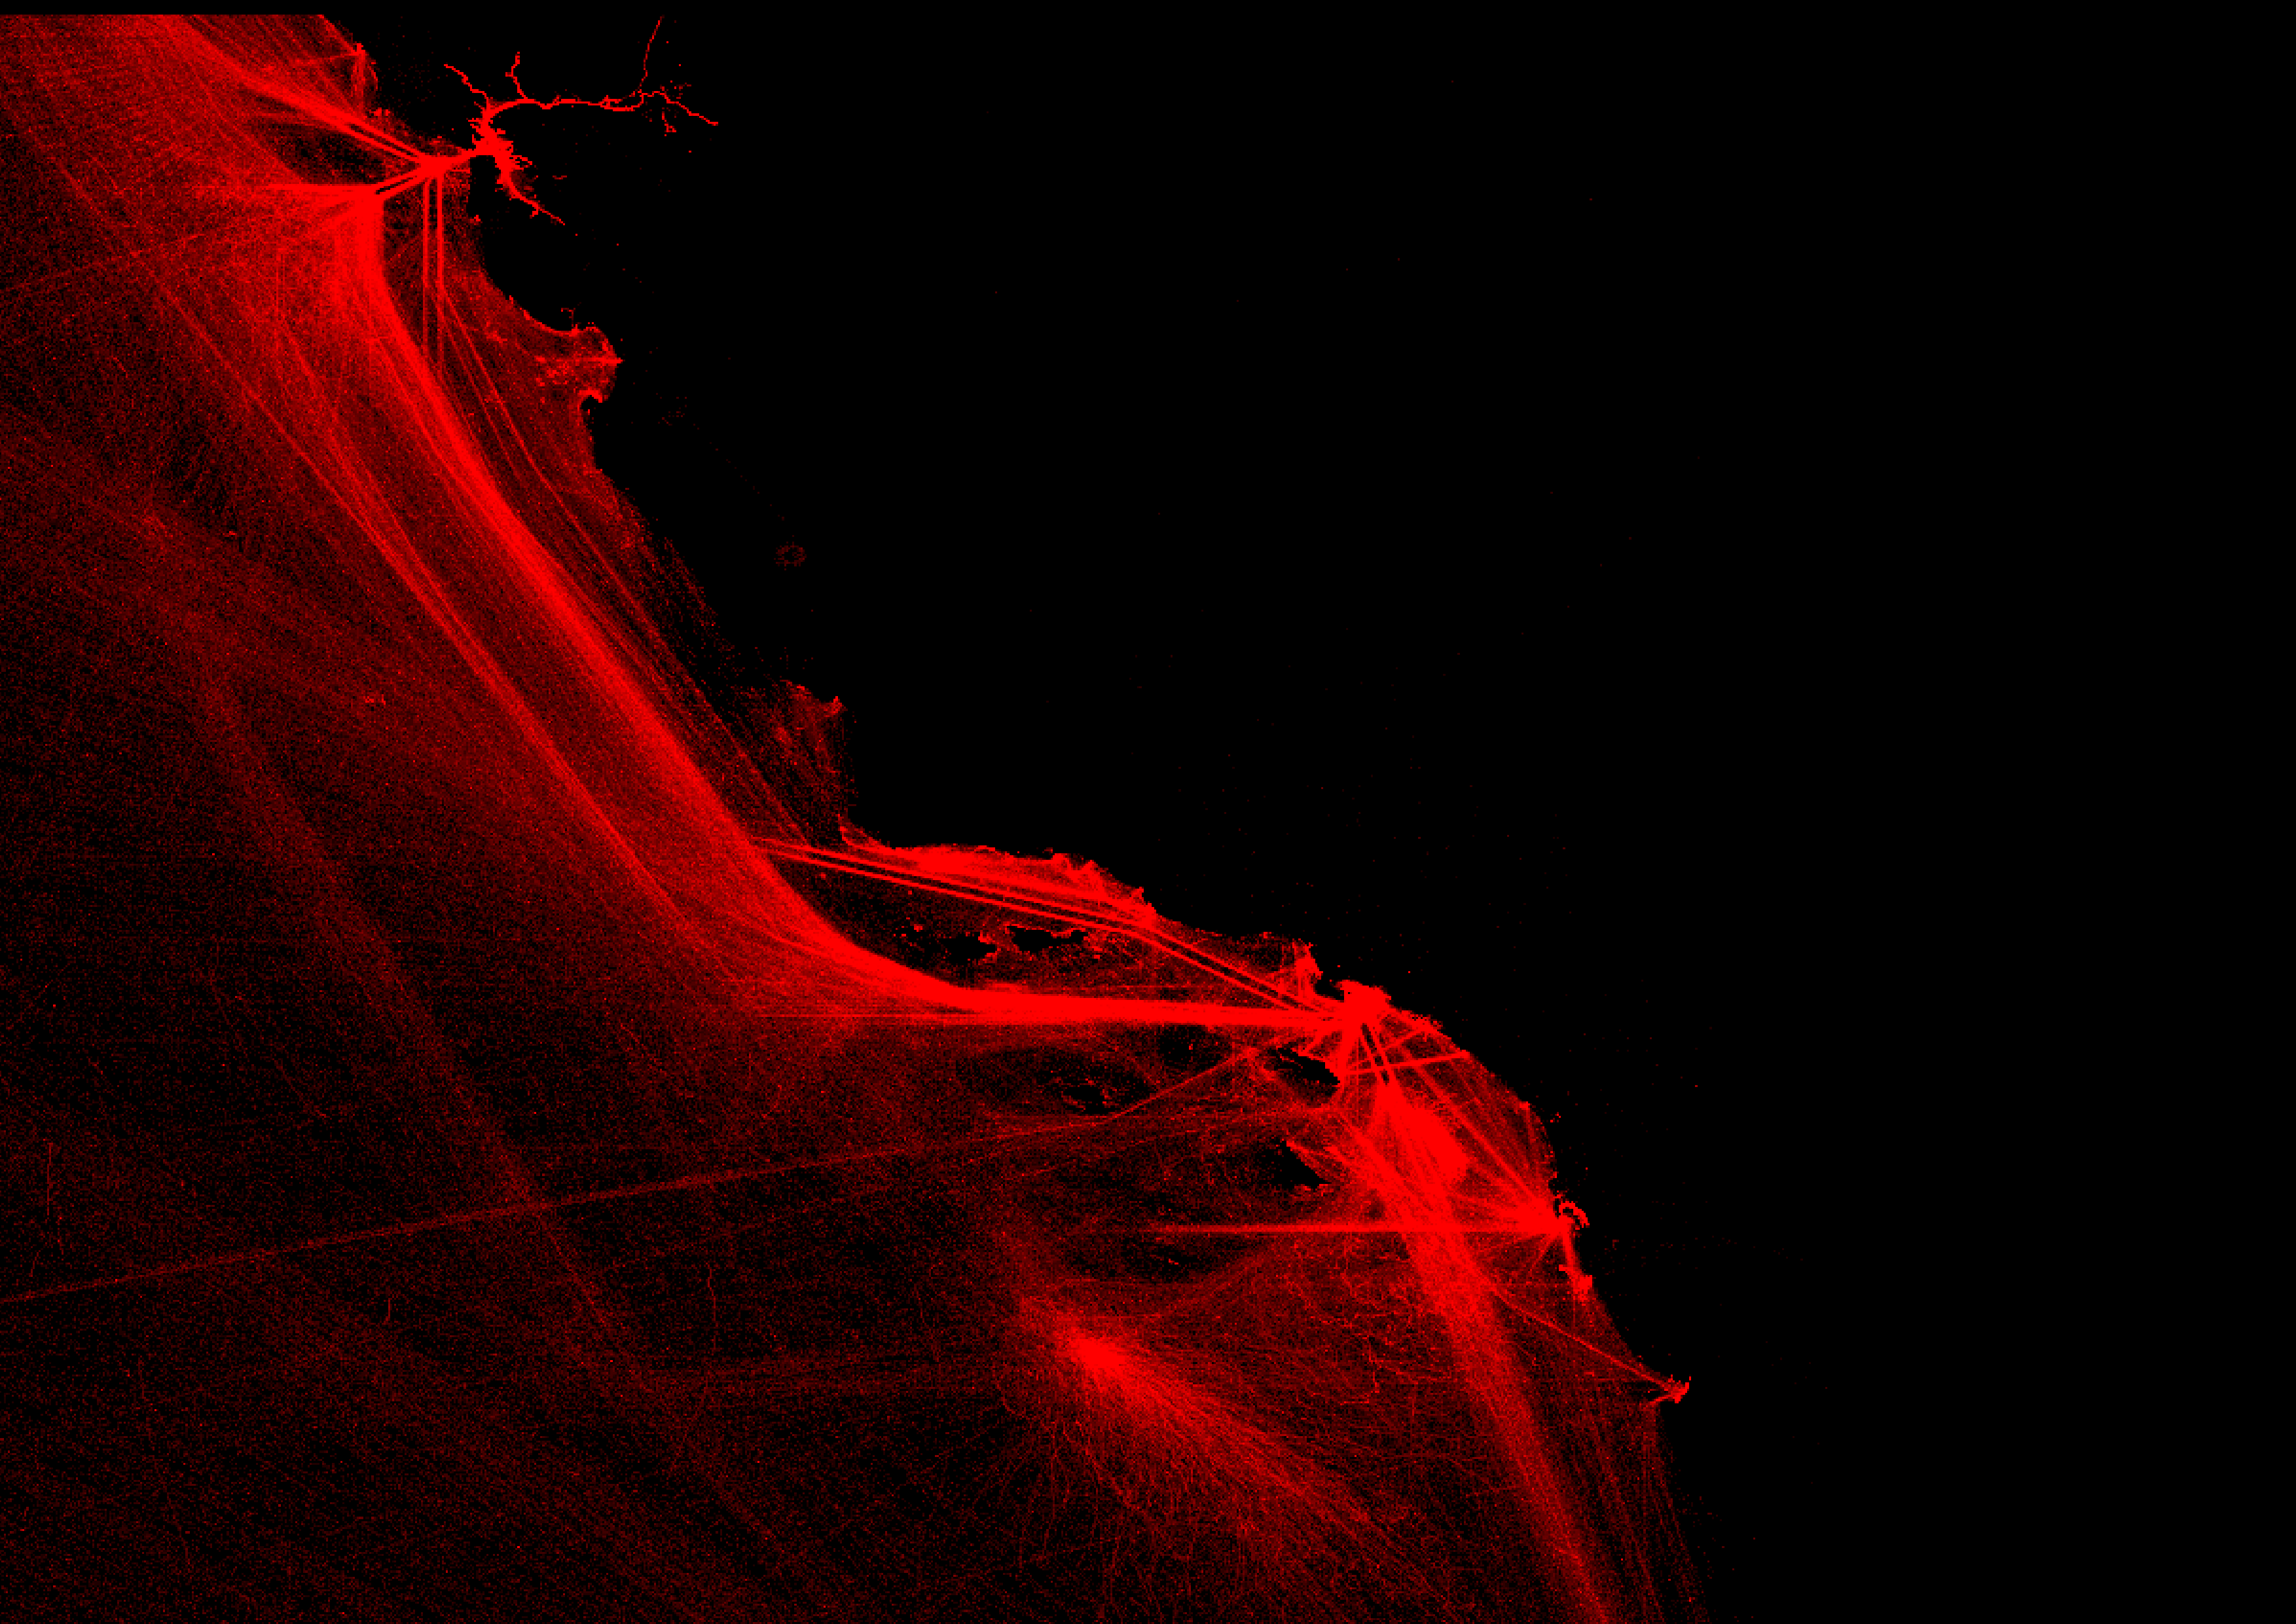
\includegraphics[width=140mm]{figures/cargo_density.png}
  \caption[AIS Observations, Southern California Bight]{AIS observations, Southern California Bight. Nov 2010--Dec 2011. Note the ballast water exchange point lower left.}
  \label{fig:cal-cargo}
\end{figure}

\begin{figure}[htbp]
  \centering
  \includegraphics[width=160mm]{figures/ais-and-ports-cea.pdf}
  \caption[AIS coverage]{Approximate AIS coverage (green), global ports (red).}
  \label{fig:ais-coverage}
\end{figure}

\begin{figure}[htbp]
  \centering
  \includegraphics[width=160mm]{figures/cia-lanes-small-cropped.png}
  \caption[CIA World Shipping Lanes]{"World Shipping Lanes" map produced by the Central Intelligence Agency, 1973.}
  \label{fig:cia-shipping-map}
\end{figure}



\ssp
% bibliography can be single-spaced for UC thesis format
%\bibliography{Library}
%\bibliographystyle{siam}
\end{document}
